\chapter{}

Something about the previous scattering results...

\begin{figure}[h!] 
  \centering
    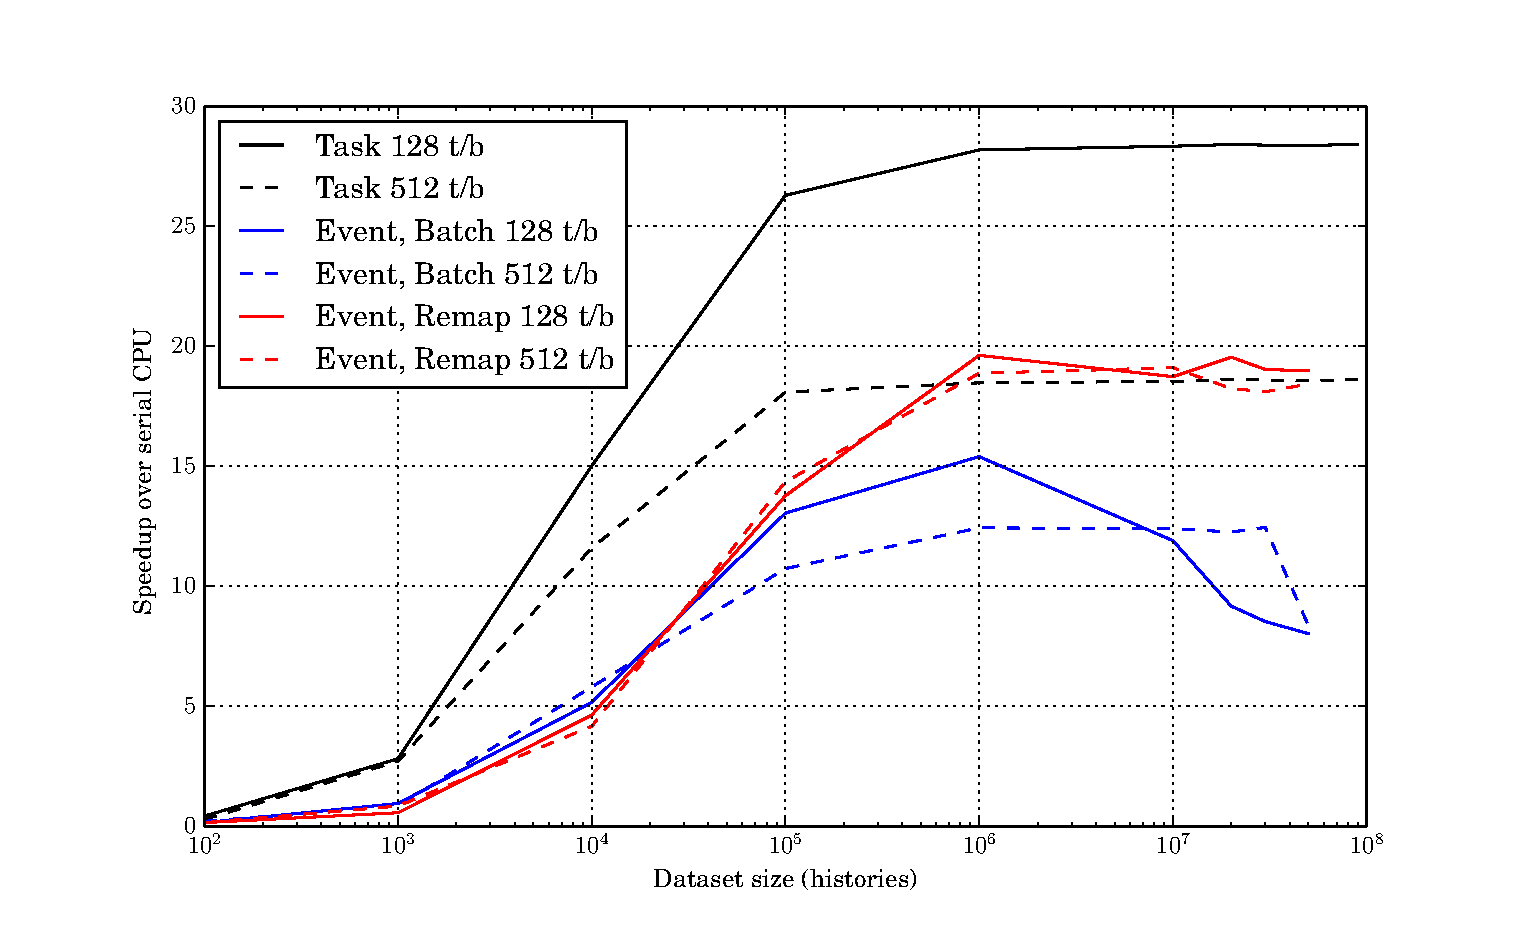
\includegraphics[width=0.8\textwidth]{graphics/prelim_speedup_old.eps}
     \caption{Speedup factors of the GPU implementations over the CPU implementation on a Tesla C2075. \label{prelim_speedup_old} }
\end{figure}

Figure \ref{prelim_speedup_old} shows the speedup factors, $F_s=t_\mathrm{CPU}/t_\mathrm{GPU}$, of the GPU implementations over the CPU implementation versus the number of particles run.  This benchmark was run on a server with a 8-core AMD Opteron 6128 CPU clocked at 2.0GHz, and there different NVIDIA cards - a Tesla K20, a Tesla C2075, and a GeForce 480 GTX.  The following results were obtained from running the GPU implementations on the Teslta K20.  The task-parallel implementation performs best, with a maximum speedup of around 29x.  The remapping implementation has the next best performance, with about a 20x speedup over the CPU.  It's performance plateaus, unlike the batched event-based implementation.  It's performance departs from the remapping implementation at $10^5$ particles and even starts to deteriorate between $10^6$ and $10^7$ particles.  This is due to the transport having to be done in batches at this point.  The simulations were done on a Tesla C2075 card, which has Fermi architecture and a maximum block number of 65,536 for a 1D grid.  Multiplying this by 128 or 512 threads per block gives maximum total number of threads of 8,388,608 and 33,554,432, respectively.  These numbers are where the batching implementation must break the transport into multiple batches.  This is also where the task-based implementation must break transport into batches, but the effect is unnoticeable since it only implies a second kernel launch instead of hundreds more.  This limit was lifted in devices with compute capability of 3.0 and up, where the maximum 1D grid size was increased to ($10^{27}-1$) \cite{cuda}.  The speedup plot also shows another important feature - that speedup plateaus at a large number of histories.  This is due to the car'd ability to hide memory latencies through pipelining when there are many many active threads.  

The most likely reasons that the task-based implementation outperforms the event-based is due the simplicity of the problem and the communication and setup overhead associated with many kernels being launched from the host.  Since the problem is so simple, all the data fits into local memory and the latencies associated with accessing global memory often are hidden.  The purpose of this study was to eliminate memory transaction and only focus on thread divergence, but memory transactions will have a very large impact when real cross sections and geometries are used.  Also only having two reactions means threads only diverge when they terminate.  WARP will have many reactions types to deal with, and divergence will be a greater problem.  This also allows threads in a block to almost always be in the same step of the transport algorithm, further eliminating divergence implicitly.  Despite this, the study does show that control flow divergence is greatly reduced by using an event-based algorithm, as shown by Figure \ref{prelim_divergence}.  The overhead of calling kernels many times in the event-based implementations is most likely the reason for the poorer performances.  It should also be noted that compiling the tests with compute capacity 2.0 (-arch sm\_20 compiler flag) improved performance about 20\% over compiling with compute capacity 3.0.